\section{Graph}

\begin{frame}[fragile]{Graph}
  \begin{adjustbox}{max totalsize={.9\textwidth}{.7\textheight},center}
    \tikzstyle{every node}=[circle, draw, fill=black!50,
    inner sep=0pt, minimum width=4pt]
    % Tutte's 8-cage
    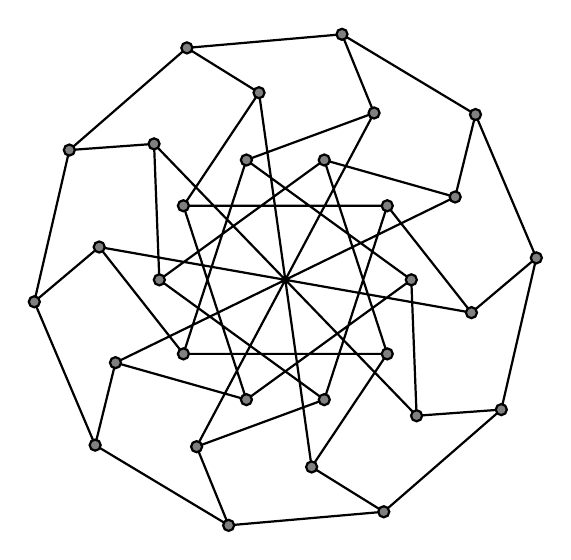
\begin{tikzpicture}[thick,scale=0.8]
      \draw \foreach \x in {0,36,...,324}
      {
        (\x:2) node {}  -- (\x+108:2)
        (\x-10:3) node {} -- (\x+5:4)
        (\x-10:3) -- (\x+36:2)
        (\x-10:3) --(\x+170:3)
        (\x+5:4) node {} -- (\x+41:4)
      };
    \end{tikzpicture}\quad

    % The largest 3-regular graph of diameter 3
    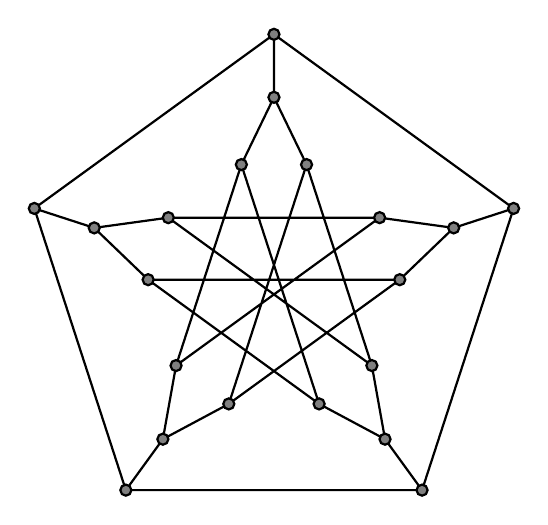
\begin{tikzpicture}[thick,scale=0.8]%
      \draw \foreach \x in {18,90,...,306} {
        (\x:4) node{} -- (\x+72:4)
        (\x:4) -- (\x:3) node{}
        (\x:3) -- (\x+15:2) node{}
        (\x:3) -- (\x-15:2) node{}
        (\x+15:2) -- (\x+144-15:2)
        (\x-15:2) -- (\x+144+15:2)
      };
    \end{tikzpicture}
  \end{adjustbox}
\end{frame}

\begin{frame}[fragile]{Content}
  \begin{easylist} \easyitem
    & 图的定义
    & 图的存储表示
    & 图的遍历
    & 图的连通性
  \end{easylist}
\end{frame}

\begin{frame}[fragile]
  \frametitle{图(Graph)}
  \begin{itemize}
  \item 图$G=(V, E)$, $V$是顶点(Vertex)集合,$E$是边/弧(Edge/Arc)的集合.
  \item 顶点的度、出度和入度
  \end{itemize}

  \begin{columns}[T]
    \column{0.5\textwidth}
    有向图:
    
    \begin{tikzpicture}[scale=1.0]
      \GraphInit[vstyle=Art]
      \Vertex{A}
      \Vertex[x=4,y=0]{B}
      \Vertex[x=0,y=2]{C}
      \Vertex[x=4,y=2]{D}
      \Edge[style={-Latex}](A)(D)

      \Edges[style={-Latex}](A,B,C, D)
      \Edges[style={-Latex}](A, C)
    \end{tikzpicture}
    
    \column{0.5\textwidth}
    无向图:
    
    \begin{tikzpicture}[scale=1.0]
      \GraphInit[vstyle=Art]
      \Vertex{A}
      \Vertex[x=4,y=0]{B}
      \Vertex[x=0,y=2]{C}
      \Vertex[x=4,y=2]{D}
      \Edge[style={}](A)(D)

      \Edges[style={}](A,B,C, D)
      \Edges[style={}](A, C)
    \end{tikzpicture}
  \end{columns}
\end{frame}

\begin{frame}[fragile]
  \frametitle{图的相关概念}
  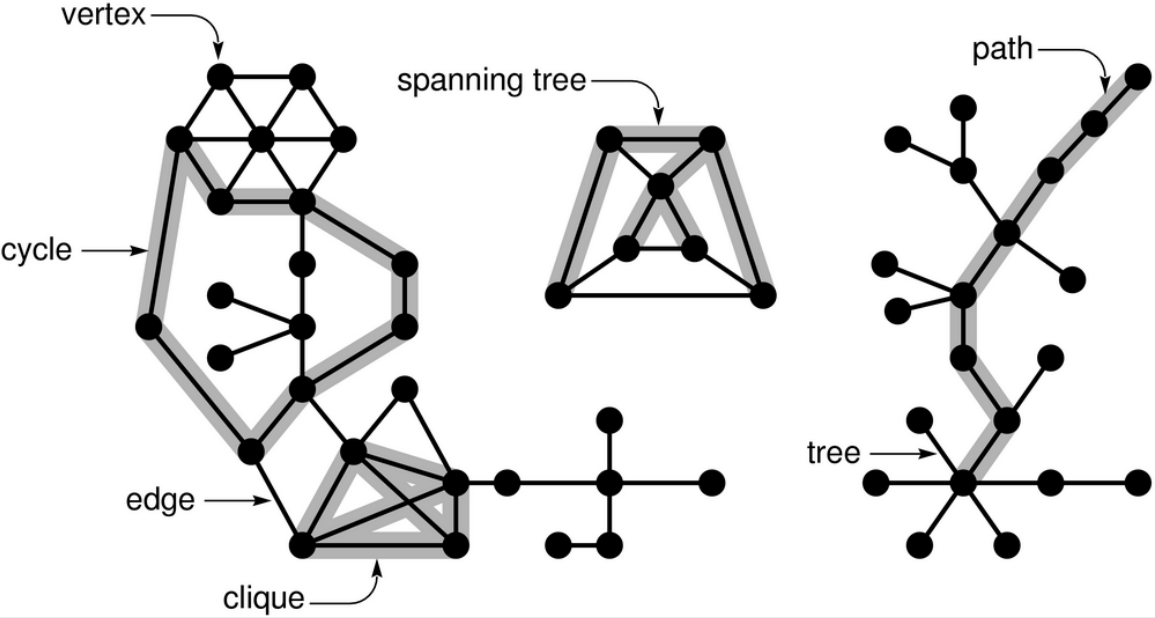
\includegraphics[width=0.9\textwidth]{figs/graph_concept.png}
\end{frame}

\begin{frame}[plain]
~  
\end{frame}

\begin{frame}[fragile]
  \frametitle{图的存储}
  如何表达下图的信息?
  \begin{columns}
    \column{0.4\textwidth}
    有向图:
    
    \begin{tikzpicture}[scale=1.3]
      \GraphInit[vstyle=Normal]
      \begin{scope}[rotate=180]
        \Vertices{circle}{$v_1$, $v_2$, $v_3$, $v_4$}
      \end{scope}
      \Edges[style={-Latex}]($v_1$,  $v_3$, $v_4$, $v_1$, $v_2$)
    \end{tikzpicture}
    
    \column{0.4\textwidth}
    无向图:
    
    \begin{tikzpicture}[scale=1.5]
      \GraphInit[vstyle=Normal]
      \begin{scope}[rotate=180]
        \Vertices{circle}{$v_1$, $v_2$, $v_3$, $v_4$}
      \end{scope}
      \Vertex{$v_5$}
      \Edges($v_1$, $v_2$, $v_3$, $v_4$, $v_1$)
      \Edges($v_2$, $v_5$, $v_3$)
    \end{tikzpicture}
  \end{columns}
  
  \pause
  \begin{itemize}
  \item 可用邻接矩阵表达顶点及其关系。
  \end{itemize}
\end{frame}


\begin{frame}[fragile]
  \frametitle{图的存储}
  \small
  \begin{columns}[T]
    \column{0.4\textwidth}
    \begin{tikzpicture}[scale=1]
      \GraphInit[vstyle=Normal]
      \begin{scope}[rotate=180]
        \Vertices{circle}{$v_1$, $v_2$, $v_3$, $v_4$}
      \end{scope}
      \Edges[style={-Latex}]($v_1$,  $v_3$, $v_4$, $v_1$, $v_2$)
    \end{tikzpicture}
    \[
      \begin{blockarray}{ccccc}
         & v_1 & v_2 & v_3 & v_4 \\
        \begin{block}{c (c c c c)}
          v_1 & 0 & 1 & 1 & 0 \\
          v_2 & 0 & 0 & 0 & 0 \\
          v_3 & 0 & 0 & 0 & 1 \\
          v_4 & 1 & 0 & 0 & 0 \\
        \end{block}
      \end{blockarray}
    \]

    \column{0.4\textwidth}
    \begin{tikzpicture}[scale=1.0]
      \GraphInit[vstyle=Normal]
      \begin{scope}[rotate=180]
        \Vertices{circle}{$v_1$, $v_2$, $v_3$, $v_4$}
      \end{scope}
      \Vertex{$v_5$}
      \Edges($v_1$, $v_2$, $v_3$, $v_4$, $v_1$)
      \Edges($v_2$, $v_5$, $v_3$)
    \end{tikzpicture}

    \[
      \begin{blockarray}{cccccc}
         & v_1 & v_2 & v_3 & v_4 & v_5 \\
        \begin{block}{c (c c c c c)}
          v_1 & 0 & 1 & 0 & 1 & 0 \\
          v_2 & 1 & 0 & 1 & 0 & 1 \\
          v_3 & 0 & 1 & 0 & 1 & 1 \\
          v_4 & 1 & 0 & 1 & 0 & 0 \\
          v_5 & 0 & 1 & 1 & 0 & 0 \\
        \end{block}
      \end{blockarray}
    \]    
  \end{columns}
  
  \begin{itemize}
  \item 根据邻接矩阵,如何判断各顶点的度?
  \end{itemize}
\end{frame}

\begin{frame}[fragile]
  \frametitle{有向图的连续存储方式:邻接矩阵}
  \begin{columns}[T]
    \column{0.4\textwidth}
    \begin{tikzpicture}[scale=1.4]
      \GraphInit[vstyle=Normal]
      \begin{scope}[rotate=180]
        \Vertices{circle}{$v_1$, $v_2$, $v_3$, $v_4$}
      \end{scope}
      \Edges[style={-Latex}]($v_1$,  $v_3$, $v_4$, $v_1$, $v_2$)
    \end{tikzpicture}
    \[
      \begin{blockarray}{ccccc}
        & v_1 & v_2 & v_3 & v_4 \\
        \begin{block}{c (c c c c)}
          v_1 & 0 & 1 & 1 & 0 \\
          v_2 & 0 & 0 & 0 & 0 \\
          v_3 & 0 & 0 & 0 & 1 \\
          v_4 & 1 & 0 & 0 & 0 \\
        \end{block}
      \end{blockarray}
    \]
    
    \column{0.6\textwidth}
    \begin{itemize}
    \item 建立二维数组$A[n][n]$, $n=|V|$
    \item 另需存放$n$个顶点信息
    \end{itemize}
  \end{columns}
\end{frame}

\begin{frame}[fragile]
  \frametitle{网的邻接矩阵}
  \begin{columns}[T]
    \column{0.4\textwidth}
    \begin{tikzpicture}[scale=1.8]
      \GraphInit[vstyle=Normal]
      \begin{scope}[rotate=180]
        \Vertices{circle}{v1, v2, v3, v4}
      \end{scope}
      \Edge[label = 8, style={-Latex}](v1)(v2)
      \Edge[label = 3, style={-Latex}](v1)(v3)
      \Edge[label = 5, style={-Latex}](v4)(v1)
      \Edge[label = 1, style={-Latex}](v3)(v4)
    \end{tikzpicture}
    \[
      \begin{blockarray}{ccccc}
        & v_1 & v_2 & v_3 & v_4 \\
        \begin{block}{c (c c c c)}
          v_1 & \infty & 8 & 3 & \infty \\
          v_2 & \infty & \infty & \infty & \infty \\
          v_3 & \infty & \infty & \infty & 1 \\
          v_4 & 5 & \infty & \infty & \infty \\
        \end{block}
      \end{blockarray}
    \]
    
    \column{0.6\textwidth}
    \begin{itemize}
    \item 有些图的边带有权重(常用来表示成本、距离、时间等), 这样的图称为:{\color{red} 网}。
    \item 网的邻接矩阵表达权重,没有边的顶点之间的权重默认为$\infty$
    \item 邻接矩阵表示方法非常直观、简单,但是会有什么问题? \pause
    \item 现实中的图经常对应稀疏矩阵,在这样情形下会有很大空间浪费.
    \end{itemize}
  \end{columns}  
\end{frame}

\begin{frame}[fragile]
  \frametitle{邻接表 (Adjacency List) -- 无向图}
  \begin{columns}[T]
    \column{0.35\textwidth}
    \begin{tikzpicture}[scale=1.3]
      \GraphInit[vstyle=Normal]
      \begin{scope}[rotate=90]
        \Vertices{circle}{v1, v2, v3, v4}
      \end{scope}
      \Edges(v3, v1, v2, v4)
    \end{tikzpicture}
    
    \column{0.6\textwidth}
    \scalebox{0.8}{
      \begin{tikzpicture}[ n/.style={minimum height=0.8cm, minimum width=1cm},
        n2/.style={minimum height=0.6cm, minimum width=1cm, fill=red!5},
        e/.style={->, very thick}]
        \draw node[n] (n0) {索引} node[n,right=0 of n0](label) {头节点};

        \foreach \x  [evaluate = \x as \xp using int(\x-1)] in {1, ..., 4}
        \draw node[n, below=0 of n\xp](n\x) {$\xp$};

        \foreach \x/\y/\z in {1/A/,2/B/,3/C/,4/D/}
        \draw node[n, right=0 of n\x, draw, fill=yellow!10](\y) {$v_\x$} node[n, right=0 of \y, draw] (P\y) {\z};


        \draw node[n2, draw, right=of PA] (c11) {2} node[n2, draw, right=0 of c11] (c12) {};
        \draw node[n2, draw, right=of c12] (c21) {1} node[n2, draw, right=0 of c21] (c22) {$\wedge$};
        \draw[e] (PA.center) -- (c11);
        \draw[e] (c12.center)--(c21);				

        \draw node[n2, draw, right=of PB] (c11) {3} node[n2, draw, right=0 of c11] (c12) {};
        \draw node[n2, draw, right=of c12] (c21) {0} node[n2, draw, right=0 of c21] (c22) {$\wedge$};
        \draw[e] (PB.center) -- (c11) (c12.center)--(c21);				

        \draw node[n2, draw, right=of PC] (c11) {0} node[n2, draw, right=0 of c11] (c12) {$\wedge$};
        \draw[e] (PC.center) -- (c11);

        \draw node[n2, draw, right=of PD] (c11) {1} node[n2, draw, right=0 of c11] (c12) {$\wedge$};
        \draw[e] (PD.center) -- (c11);
      \end{tikzpicture}
    }
  \end{columns}

  \begin{itemize}
  \item 无向图的邻接表:同一个顶点发出的边链接在同一个边链表中,便于确定顶点的度
  \item 需要$n$个头结点, $2e$个表结点
  \end{itemize}
\end{frame}

\begin{frame}[fragile]
  \frametitle{邻接表--有向图}
  \begin{columns}[T]
    \column{0.4\textwidth}
    \begin{tikzpicture}[scale=1.5]
      \GraphInit[vstyle=Normal]
      \begin{scope}[rotate=135]
        \Vertices{circle}{A, B, C, E}
      \end{scope}
      \Vertex{D}
      \Edges[style={-Latex}](A, B, C, D, E, A)
      \Edge[style={-Latex}](A)(D)	
    \end{tikzpicture}
    
    邻接表,便于确定节点出度

    \scalebox{0.7}{
      \begin{tikzpicture}[ n/.style={minimum height=0.8cm, minimum width=1cm},
        n2/.style={minimum height=0.6cm, minimum width=1cm, fill=red!5},
        e/.style={->, very thick}]
        \draw node[n] (n0) {索引} node[n,right=0 of n0](label) {头节点};

        \foreach \x  [evaluate = \x as \xp using int(\x-1)] in {1, ..., 5}
        \draw node[n, below=0 of n\xp](n\x) {$\xp$};

        \foreach \x/\y/\z in {1/A/,2/B/,3/C/,4/D/, 5/E/}
        \draw node[n, right=0 of n\x, draw, fill=yellow!10](\y) {$\y$} node[n, right=0 of \y, draw] (P\y) {\z};


        \draw node[n2, draw, right=of PA] (c11) {3} node[n2, draw, right=0 of c11] (c12) {};
        \draw node[n2, draw, right=of c12] (c21) {1} node[n2, draw, right=0 of c21] (c22) {$\wedge$};
        \draw[e] (PA.center) -- (c11);
        \draw[e] (c12.center)--(c21);				

        \draw node[n2, draw, right=of PB] (c11) {2} node[n2, draw, right=0 of c11] (c12) {$\wedge$};
        \draw[e] (PB.center) -- (c11);

        \draw node[n2, draw, right=of PC] (c11) {3} node[n2, draw, right=0 of c11] (c12) {$\wedge$};
        \draw[e] (PC.center) -- (c11);

        \draw node[n2, draw, right=of PD] (c11) {4} node[n2, draw, right=0 of c11] (c12) {$\wedge$};
        \draw[e] (PD.center) -- (c11);

        \draw node[n2, draw, right=of PE] (c11) {0} node[n2, draw, right=0 of c11] (c12) {$\wedge$};
        \draw[e] (PE.center) -- (c11);
      \end{tikzpicture}
    }
    \pause
    
    \column{0.6\textwidth}
    逆邻接表,便于确定节点入度
    
    \scalebox{0.7}{
      \begin{tikzpicture}[ n/.style={minimum height=0.8cm, minimum width=1cm},
        n2/.style={minimum height=0.6cm, minimum width=1cm, fill=red!5},
        e/.style={->, very thick}]
        \draw node[n] (n0) {索引} node[n,right=0 of n0](label) {头节点};

        \foreach \x  [evaluate = \x as \xp using int(\x-1)] in {1, ..., 5}
        \draw node[n, below=0 of n\xp](n\x) {$\xp$};

        \foreach \x/\y/\z in {1/A/,2/B/,3/C/,4/D/, 5/E/}
        \draw node[n, right=0 of n\x, draw, fill=yellow!10](\y) {$\y$} node[n, right=0 of \y, draw] (P\y) {\z};

        \draw node[n2, draw, right=of PA] (c11) {4} node[n2, draw, right=0 of c11] (c12) {$\wedge$};
        \draw[e] (PA.center) -- (c11);

        \draw node[n2, draw, right=of PB] (c11) {0} node[n2, draw, right=0 of c11] (c12) {$\wedge$};
        \draw[e] (PB.center) -- (c11);

        \draw node[n2, draw, right=of PC] (c11) {1} node[n2, draw, right=0 of c11] (c12) {$\wedge$};
        \draw[e] (PC.center) -- (c11);

        \draw node[n2, draw, right=of PD] (c11) {2} node[n2, draw, right=0 of c11] (c12) {};
        \draw node[n2, draw, right=of c12] (c21) {0} node[n2, draw, right=0 of c21] (c22) {$\wedge$};
        \draw[e] (PD.center) -- (c11);
        \draw[e] (c12.center)--(c21);		

        \draw node[n2, draw, right=of PE] (c11) {3} node[n2, draw, right=0 of c11] (c12) {$\wedge$};
        \draw[e] (PE.center) -- (c11);
      \end{tikzpicture}
    }    
  \end{columns}
\end{frame}

\begin{frame}[fragile]
  \frametitle{邻接表--权重处理}
  \scalebox{0.7}{
    \begin{tikzpicture}[scale=2]
      \GraphInit[vstyle=Normal]
      \begin{scope}[rotate=225]
        \Vertices{circle}{A, B, D, C}
      \end{scope}

      \Edge[style={-Latex}, label=1](A)(B)
      \Edge[style={-Latex, pos=0.2}, label=4](A)(D)

      \Edge[style={-Latex, pos=0.2, bend right}, label=9](B)(C)
      \Edge[style={-Latex}, label=2](B)(D)

      \Edge[style={-Latex}, label=3](C)(A)
      \Edge[style={-Latex, pos=0.2, bend right=10}, label=5](C)(B)
      \Edge[style={-Latex}, label=8](C)(D)

      \Edge[style={-Latex, bend right=40}, label=6](D)(C)
    \end{tikzpicture}
  }

  \scalebox{0.7}{
    \begin{tikzpicture}[ n/.style={minimum height=0.8cm, minimum width=1cm},
      n2/.style={minimum height=0.6cm, minimum width=1cm, fill=red!5},
      e/.style={->, very thick}]
      \draw node[n] (n0) {索引} node[n,right=0 of n0](label) {头节点};

      \foreach \x  [evaluate = \x as \xp using int(\x-1)] in {1, ..., 4}
      \draw node[n, below=0 of n\xp](n\x) {$\xp$};

      \foreach \x/\y/\z in {1/A/,2/B/,3/C/,4/D/}
      \draw node[n, right=0 of n\x, draw, fill=yellow!10](\y) {$\y$} node[n, right=0 of \y, draw] (P\y) {\z};

      \draw node[n2, draw, right=of PA] (c11) {1} node[n2, draw, right=0 of c11,fill=blue!10] (c12) {1} node[n2, draw, right=0 of c12] (c13) {};
      \draw node[n2, draw, right=of c13] (c21) {3}  node[n2, draw, right=0 of c21,fill=blue!10] (c22) {4} node[n2, draw, right=0 of c22] (c23) {$\wedge$};
      \draw[e] (PA.center) -- (c11);
      \draw[e] (c13.center) -- (c21);

      \draw node[above=of c11](tip1) {边的终点} node[right=of tip1](tip2){权重};
      \path[draw, ->] (tip1) edge (c11) (tip2) edge[bend right] (c12);
      
      \draw node[n2, draw, right=of PB] (c11) {3} node[n2, draw, right=0 of c11,fill=blue!10] (c12) {2} node[n2, draw, right=0 of c12] (c13) {};
      \draw node[n2, draw, right=of c13] (c21) {2}  node[n2, draw, right=0 of c21,fill=blue!10] (c22) {9} node[n2, draw, right=0 of c22] (c23) {$\wedge$};
      \draw[e] (PB.center) -- (c11);
      \draw[e] (c13.center) -- (c21);

      \draw node[n2, draw, right=of PC] (c11) {0} node[n2, draw, right=0 of c11,fill=blue!10] (c12) {3} node[n2, draw, right=0 of c12] (c13) {};
      \draw node[n2, draw, right=of c13] (c21) {1}  node[n2, draw, right=0 of c21,fill=blue!10] (c22) {5} node[n2, draw, right=0 of c22] (c23) {};
      \draw node[n2, draw, right=of c23] (c31) {3}  node[n2, draw, right=0 of c31,fill=blue!10] (c32) {8} node[n2, draw, right=0 of c32] (c33) {$\wedge$};
      \draw[e] (PC.center) -- (c11);
      \draw[e] (c13.center) -- (c21);
      \draw[e] (c23.center) -- (c31);

      \draw node[n2, draw, right=of PD] (c11) {2} node[n2, draw, right=0 of c11,fill=blue!10] (c12) {6} node[n2, draw, right=0 of c12] (c13) {$\wedge$};
      \draw[e] (PD.center) -- (c11);
    \end{tikzpicture}
  }
\end{frame}

\begin{frame}[fragile]
  \frametitle{练习}
  \begin{enumerate}
  \item 请写出数组存储和邻接表的类型定义
  \item 请在如下方面对比数组表示法和邻接表示法
    \begin{itemize}
    \item 存储表示是否唯一
    \item 空间复杂度
    \item 操作a: 求顶点$v_i$的度
    \item 操作b: 判定$(v_i, v_j)$是否是图的一条边
    \item 操作c: 通过遍历求边的数目
    \end{itemize}
  \end{enumerate}
\end{frame}
% TODO

\begin{frame}[fragile, allowframebreaks]
  \frametitle{邻接表表示}
  \begin{minted}{java}
    class VertexNode {
      String data;
      EdgeNode firstAdj = null;

      public VertexNode(String data) {
        this.data = data;
      }
    }

    class EdgeNode {
      int adjVertexNode;
      EdgeNode nextAdj = null;

      public EdgeNode(int vertexIdx) {
        this.adjVertexNode = vertexIdx;
      }

      public EdgeNode(int vertexIdx, EdgeNode nextAdj) {
        this.adjVertexNode = vertexIdx;
        this.nextAdj = nextAdj;
      }
    }
    
    public class Graph {
      VertexNode[] vertices;

      public void init() {
        this.vertices = new VertexNode[]{
          new VertexNode("v1"),
          new VertexNode("v2"),
          new VertexNode("v3"),
          new VertexNode("v4"),
          new VertexNode("v5"),
          new VertexNode("v6"),
          new VertexNode("v7"),
          new VertexNode("v8")
        };
        vertices[0].firstAdj = new EdgeNode(1, new EdgeNode(2));
        vertices[1].firstAdj = new EdgeNode(0, new EdgeNode(3, new EdgeNode(4)));
        vertices[2].firstAdj = new EdgeNode(0, new EdgeNode(5, new EdgeNode(6)));
        vertices[3].firstAdj = new EdgeNode(1, new EdgeNode(7));
        vertices[4].firstAdj = new EdgeNode(1, new EdgeNode(7));
        vertices[5].firstAdj = new EdgeNode(2, new EdgeNode(6));
        vertices[6].firstAdj = new EdgeNode(2, new EdgeNode(5));
        vertices[7].firstAdj = new EdgeNode(3, new EdgeNode(4));
      }
    }
  \end{minted}
\end{frame}

\begin{frame}[fragile]
  \frametitle{比较}
  \small
  \begin{tabular}{| p{2cm} | p{4cm} | p{4cm} |}
    \hline
    ~ & 数组表示法 & 邻接表法 \\ \hline
    表示结果 & 唯一 & 不唯一 \\ \hline
    空间复杂度 & $O(n^2)$ (适用于稠密图) & $O(n+e)$ (适用于稀疏图) \\ \hline
    无向图求顶点$v_i$的度 & 第$i$行(或第$i$列)上非零元素的个数 & 第$i$个边表中的结点个数 \\ \hline
    有向图求顶点$v_i$的度  & 第$i$行上非零元素的个数是$v_i$出度,第$i$列上非零元素的个数是$v_i$的入度 & 第$i$个边表上的结点个数,求入度还需遍历各顶点的边表。逆邻接表则相反\\ \hline
    判定$(v_i, v_j)$是否是图的一条边 &  看矩阵中的$i$行$j$列是否为0 & 扫描第i个边表 \\ \hline
    求边的数目 & 检测整个矩阵中的非零元所耗费的时间是$O(N^2)$ & 对每个边表的结点个数计数所耗费的时间是$O(e+n)$ \\ \hline
  \end{tabular}  
\end{frame}

\begin{frame}[fragile]
  \frametitle{思考}

  怎么把邻接表和逆邻接表相结合,同时表示出来?
\end{frame}

\begin{frame}[fragile]
  \frametitle{有向图的十字链表(Orthogonal List)}
  \begin{columns}[T]
    \column{0.4\textwidth}
    \begin{tikzpicture}[scale=1.2]
      \GraphInit[vstyle=Normal]
      \SetVertexMath
      \begin{scope}[rotate=135]
        \Vertices{circle}{A, C, D, B}
      \end{scope}
      \Edges[style={-Latex}](C,D,A,B)
      \Edges[style={-Latex}](D,B)
      \Edges[style={-Latex, bend left}](C,A,C)
    \end{tikzpicture}

    \column{0.6\textwidth}
    将邻接表、逆邻接表结合起来.
    \begin{itemize}
    \item hlink: 指向弧头相同的下一条弧
    \item tlink: 指向弧尾相同的下一条弧
    \end{itemize}
  \end{columns}
  \scalebox{0.7}{
    \begin{tikzpicture}[ n/.style={minimum height=0.8cm, minimum width=1cm},
      n2/.style={minimum height=0.6cm, minimum width=1cm, fill=red!5},
      n3/.style={minimum height=0.6cm, minimum width=1cm},
      e/.style={->, thick, red},
      e2/.style={->, thick, blue}]
      \draw node[n] (n0) {索引} node[n,right=0 of n0](label) {头节点};

      \foreach \x  [evaluate = \x as \xp using int(\x-1)] in {1, ..., 4}
      \draw node[n, below=0 of n\xp](n\x) {$\xp$};

      \foreach \x/\y/\z/\v in {1/A//,2/B//,3/C//,4/D//}
      \draw node[n, right=0 of n\x, draw, fill=yellow!10](\y) {$\y$} node[n, right=0 of \y, draw] (firstIn\y) {\z} node[n, right=0 of firstIn\y, draw] (firstOut\y) {\v};

      \draw node[n2, draw, right=of firstOutA] (headAB) {0} node[n2, draw, right=0 of headAB] (tailAB) {1} node[n3, draw, right=0 of tailAB] (headLinkAB) {} node[n3, draw, right=0 of headLinkAB] (tailLinkAB) {};

      \draw node[n2, draw, right=of tailLinkAB] (headAC) {0} node[n2, draw, right=0 of headAC] (tailAC) {2} node[n3, draw, right=0 of tailAC] (headLinkAC) {} node[n3, draw, right=0 of headLinkAC] (tailLinkAC) {$\wedge$};

      \draw node[n2, draw, right=of firstOutC] (headCA) {2} node[n2, draw, right=0 of headCA] (tailCA) {0} node[n3, draw, right=0 of tailCA] (headLinkCA) {} node[n3, draw, right=0 of headLinkCA] (tailLinkCA) {};

      \draw node[n2, draw, right=of tailLinkCA] (headCD) {2} node[n2, draw, right=0 of headCD] (tailCD) {3} node[n3, draw, right=0 of tailCD] (headLinkCD) {} node[n3, draw, right=0 of headLinkCD] (tailLinkCD) {};

      \draw node[n2, draw, right=of firstOutD] (headDA) {3} node[n2, draw, right=0 of headDA] (tailDA) {0} node[n3, draw, right=0 of tailDA] (headLinkDA) {$\wedge$} node[n3, draw, right=0 of headLinkDA] (tailLinkDA) {};

      \draw node[n2, draw, right=of tailLinkDA] (headDB) {3} node[n2, draw, right=0 of headDB] (tailDB) {1} node[n3, draw, right=0 of tailDB] (headLinkDB) {} node[n3, draw, right=0 of headLinkDB] (tailLinkDB) {};

      \draw[] node[above=1.5cm of firstInA](tipFirstIn) {$firstIn$} node[right=0 of tipFirstIn] (tipFirstOut) {$firstOut$} 
      node[above=1cm of headAB] (tipHeadAB) {$tailVertex$} node[above=1.5cm of tailAB] (tipTailAB) {$headVertex$}
      node[above=1cm of headLinkAB] (tipHeadLinkAB) {$hlink$} node[right=0 of tipHeadLinkAB] (tipTailLinkAB) {$tlink$};

      % draw tip of node
      \path[draw, <-, dashed] (tipFirstIn) edge (firstInA) 
      (tipFirstOut) edge[bend right] (firstOutA)
      (tipHeadAB) edge[] (headAB)
      (tipTailAB) edge[bend left] (tailAB)
      (tipHeadLinkAB) edge[bend left] (headLinkAB)
      (tipTailLinkAB) edge[bend left] (tailLinkAB); 

      % draw links
      \path[e] (firstInA.center) edge[bend left=45, out=120] (headLinkCA.north);
      \draw[e] (headLinkCA.center) -- (headLinkDA.north);
      \draw[e2] (firstOutA.center) -- (headAB);
      \draw[e2] (tailLinkAB.center) -- (headAC);
    \end{tikzpicture}
  }
\end{frame}

\begin{frame}[fragile]
  \frametitle{有向图的十字链表}
  \begin{columns}
    \column{0.5\textwidth}
    \begin{minted}[fontsize=\small]{java}
      class VertexNode {
        String data;
        ArcBox firstIn;
        ArcBox firstOut;
      }

      class ArcBox {
        int headVertex, tailVertex;
        ArcBox hlink;
        ArcBox tlink;
        String data;
      }
    \end{minted}
    \column{0.5\textwidth}
    \begin{minted}[fontsize=\small]{java}
      class OLGraph {
        List<VertexNode> xlist;
        int vertexNum, arcNum;
      }
    \end{minted}
  \end{columns}
\end{frame}

\begin{frame}[fragile]
  \frametitle{无向图的多重邻接表}
  \begin{columns}[T]
    \column{0.3\textwidth}
    \begin{tikzpicture}[scale=1.2]
      \GraphInit[vstyle=Normal]
      \SetVertexMath
      \begin{scope}[rotate=135]
        \Vertices{circle}{v_0, v_2, v_3, v_1}
      \end{scope}
      \Edges[](v_0, v_1, v_3, v_2, v_0, v_3)
    \end{tikzpicture}

    \column{0.7\textwidth}
    \small
    \begin{itemize}
    \item 无向图的应用中,关注的重点是顶点,那么邻接表是不错的选择
    \item 如更关注边的操作,比如对已访问过的边做标记,删除某一条边等操作,就意味着需要找到这条边的两个边表结点进行操作。
    \end{itemize}
  \end{columns}

  \begin{tabular}{|c|c|c|c}
    \hline
    $ivex$ & $ilink$ & $jvex$ & $jlink$ \\ \hline
  \end{tabular}
  
  \begin{itemize}
  \item $ivex$, $jvex$: 某条边依附的两个顶点
  \item $ilink$: 指向依附顶点$ivex$的下一条边
  \item $jlink$: 指向依附顶点$jvex$的下一条边
  \end{itemize}
\end{frame}

\begin{frame}[fragile]
  \frametitle{无向图的多重邻接表}
  \begin{columns}[T]
    \column{0.3\textwidth}
    \begin{tikzpicture}[scale=1.2]
      \GraphInit[vstyle=Normal]
      \SetVertexMath
      \begin{scope}[rotate=135]
        \Vertices{circle}{v_0, v_2, v_3, v_1}
      \end{scope}
      \Edges[](v_0, v_1, v_3, v_2, v_0, v_3)
    \end{tikzpicture}

    \column{0.7\textwidth}
    \small
    \begin{itemize}
    \item 无向图的应用中,关注的重点是顶点,那么邻接表是不错的选择
    \item 如更关注边的操作,比如对已访问过的边做标记,删除某一条边等操作,就意味着需要找到这条边的两个边表结点进行操作。
    \end{itemize}
  \end{columns}

  \scalebox{0.7}{
    \begin{tikzpicture}[ n/.style={minimum height=0.8cm, minimum width=1cm},
      n2/.style={minimum height=0.6cm, minimum width=1cm, fill=red!5},
      n3/.style={minimum height=0.6cm, minimum width=1cm},
      e/.style={draw, ->, thick, red},
      e2/.style={draw, ->, thick, blue}]
      \draw node[n] (n0) {索引} node[n,right=0 of n0](label) {头节点};

      \foreach \x  [evaluate = \x as \xp using int(\x-1)] in {1, ..., 4}
      \draw node[n, below=0 of n\xp](n\x) {$\xp$};

      \foreach \x/\y/\z in {1/A/v_0,2/B/v_1,3/C/v_2,4/D/v_3}
      \draw node[n, right=0 of n\x, draw, fill=yellow!10](\y) {$\z$} node[n, right=0 of \y, draw] (firstEdge\y) {};

      \draw node[n2, draw, right=of firstEdgeA] (ivexAB) {0} node[n3, draw, right=0 of ivexAB] (ilinkAB) {} node[n2, draw, right=0 of ilinkAB] (jvexAB) {1} node[n3, draw, right=0 of jvexAB] (jlinkAB) {};
      \draw node[n2, draw, right=of jlinkAB] (ivexAC) {0} node[n3, draw, right=0 of ivexAC] (ilinkAC) {} node[n2, draw, right=0 of ilinkAC] (jvexAC) {2} node[n3, draw, right=0 of jvexAC] (jlinkAC) {};
      \draw node[n2, draw, below=0.5 of jvexAC] (ivexAD) {0} node[n3, draw, right=0 of ivexAD] (ilinkAD) {$\wedge$} node[n2, draw, right=0 of ilinkAD] (jvexAD) {3} node[n3, draw, right=0 of jvexAD] (jlinkAD) {$\wedge$};
      

      \draw node[n2, draw, right=of firstEdgeD] (ivexDB) {3} node[n3, draw, right=0 of ivexDB] (ilinkDB) {} node[n2, draw, right=0 of ilinkDB] (jvexDB) {1} node[n3, draw, right=0 of jvexDB] (jlinkDB) {};

      \draw node[n2, draw, right=of jlinkDB] (ivexDC) {3} node[n3, draw, right=0 of ivexDC] (ilinkDC) {} node[n2, draw, right=0 of ilinkDC] (jvexDC) {2} node[n3, draw, right=0 of jvexDC] (jlinkDC) {};


      \draw[] node[above=1.5cm of firstEdgeA](tipFirstEdge) {$firstEdge$}  
      node[above=1cm of ivexAB] (tipivex) {$ivex$} node[above=1.5cm of jvexAB] (tipjvex) {$jvex$}
      node[above=1cm of ilinkAB] (tipilink) {$ilink$} node[right=0 of tipjvex] (tipjlink) {$jlink$};

      \path[draw, ->, dashed] (firstEdgeA) edge (tipFirstEdge)
      (ivexAB) edge (tipivex)
      (ilinkAB) edge (tipilink)
      (jvexAB) edge (tipjvex)
      (jlinkAB) edge (tipjlink);

      \path[e] (firstEdgeA.center) -- (ivexAB);
      \draw[e] (ilinkAB.center) to[out=90,in=180] (ivexAC);
      \draw[e] (ilinkAC.center) to[out=270, in=180] (ivexAD.west);

      \path[e] (firstEdgeD.center) -- (ivexDB);
      \draw[e] (ilinkDB.center) to[out=270,in=180] (ivexDC);
      \draw[e] (ilinkDC.center) to[out=90,in=220] (ivexAD);

    \end{tikzpicture}
  }
\end{frame}

\subsection{图的遍历}
\begin{frame}[fragile]
  \frametitle{图的遍历}
  ~
\end{frame}

\begin{frame}[fragile]
  \frametitle{图的遍历}

  图的遍历:从图的某顶点出发,访问所有顶点,且每个顶点仅被访问一次。
  
  无论是无向图还是有向图,都有两种遍历方式:
  \begin{columns}[T]
    \column{0.6\textwidth}
    \begin{itemize}
    \item 深度优先(类似于树的先根遍历)
    \item 广度优先(类似于树的层次遍历)
    \end{itemize}
    
    \column{0.6\textwidth}
    \scalebox{0.7}{
      \begin{tikzpicture}[scale=1]
        \GraphInit[vstyle=Normal]
        \SetVertexMath
        \Vertex{v_1}
        \Vertex[x=-2, y=-1]{v_2}
        \Vertex[x=1.5, y=-1]{v_3}

        \SOWE(v_2){v_4}
        \SOEA(v_2){v_5}


        \SOWE(v_3){v_6}
        \SOEA(v_3){v_7}
        \SOWE(v_5){v_8}

        \Edges(v_1,v_2,v_4,v_8,v_5,v_2)
        \Edges(v_1,v_3,v_6,v_7,v_3)
      \end{tikzpicture}
    }
  \end{columns}
\end{frame}

\begin{frame}[fragile]
  \frametitle{深度优先搜索 - Depth First Search}

  \begin{columns}[T]
    \column{0.65\textwidth}
    \scalebox{0.8}{
      \begin{tikzpicture}[scale=1]
        \GraphInit[vstyle=Normal]
        \SetVertexMath
        \Vertex{v_1}
        \Vertex[x=-2, y=-1]{v_2}
        \Vertex[x=1.5, y=-1]{v_3}

        \SOWE(v_2){v_4}
        \SOEA(v_2){v_5}


        \SOWE(v_3){v_6}
        \SOEA(v_3){v_7}
        \SOWE(v_5){v_8}

        \Edges(v_1,v_2,v_4,v_8,v_5,v_2)
        \Edges(v_1,v_3,v_6,v_7,v_3)
      \end{tikzpicture}
    }

    以$v_1$开始为例:$v_1 \rightarrow v_2 \rightarrow v_4 \rightarrow v_8
    \rightarrow v_5 \rightarrow \cdots$
    
    \scalebox{0.8}{
      \begin{tikzpicture}[ n/.style={minimum size=0.8cm}]
        \draw node[] (n0) {};
        \foreach \x  [evaluate = \x as \xp using int(\x-1)] in {1, ..., 8}
        \draw node[n, right=0 of n\xp](n\x) {$v_\x$};

        \foreach \x/\y in {1/1,2/1,3/0,4/1,5/1, 6/0, 7/0, 8/1}
        \draw node[n, below=0 of n\x, draw, fill=red!5](d\x) {$\y$};

        \draw node[left=0 of d1]{$visited$};

        \foreach \x/\y in {1/v_1,2/v_2,3/v_4,4/v_8,5/v_5, 6/, 7/, 8/}
        \draw node[n, below=0.3 of d\x, draw, fill=yellow!20](d\x) {$\y$};

        \draw node[left=0 of d1]{$stack$};
      \end{tikzpicture}
    }
    
    \column{0.35\textwidth}
    \begin{tabular}{| l | l |}
      \hline
      $v_1$ & $\rightarrow v_2 \rightarrow v_3$ \\ \hline
      $v_2$ & $\rightarrow v_1 \rightarrow v_4 \rightarrow v_5$ \\ \hline
      $v_3$ & $\rightarrow v_1 \rightarrow v_6 \rightarrow v_7$ \\ \hline
      $v_4$ & $\rightarrow v_2 \rightarrow v_8$ \\ \hline
      $v_5$ & $\rightarrow v_2 \rightarrow v_8$ \\ \hline
      $v_6$ & $\rightarrow v_3 \rightarrow v_7$ \\ \hline
      $v_7$ & $\rightarrow v_3 \rightarrow v_6$ \\ \hline
      $v_8$ & $\rightarrow v_4 \rightarrow v_5$ \\ \hline      
    \end{tabular}
  \end{columns}

  \pause
  
  $v_1 \rightarrow v_2 \rightarrow v_4 \rightarrow v_8
  \rightarrow v_5$ \color{red} $\rightarrow v_3 \rightarrow v_6 \rightarrow v_7$  
\end{frame}

\begin{frame}[fragile, plain, allowframebreaks]
  %\frametitle{DFS}
  \begin{minted}[fontsize=\small]{java}
    class VertexNode {
      String data;
      EdgeNode firstAdj = null;

      public VertexNode(String data) {
        this.data = data;
      }
    }

    class EdgeNode {
      int adjVertexNode;
      EdgeNode nextAdj = null;

      public EdgeNode(int vertexIdx) {
        this.adjVertexNode = vertexIdx;
      }

      public EdgeNode(int vertexIdx, EdgeNode nextAdj) {
        this.adjVertexNode = vertexIdx;
        this.nextAdj = nextAdj;
      }
    }
    
    public class Graph {
      VertexNode[] vertices;

      public void init() {
        this.vertices = new VertexNode[]{
          new VertexNode("v1"),
          new VertexNode("v2"),
          new VertexNode("v3"),
          new VertexNode("v4"),
          new VertexNode("v5"),
          new VertexNode("v6"),
          new VertexNode("v7"),
          new VertexNode("v8")
        };
        vertices[0].firstAdj = new EdgeNode(1, new EdgeNode(2));
        vertices[1].firstAdj = new EdgeNode(0, new EdgeNode(3, new EdgeNode(4)));
        vertices[2].firstAdj = new EdgeNode(0, new EdgeNode(5, new EdgeNode(6)));
        vertices[3].firstAdj = new EdgeNode(1, new EdgeNode(7));
        vertices[4].firstAdj = new EdgeNode(1, new EdgeNode(7));
        vertices[5].firstAdj = new EdgeNode(2, new EdgeNode(6));
        vertices[6].firstAdj = new EdgeNode(2, new EdgeNode(5));
        vertices[7].firstAdj = new EdgeNode(3, new EdgeNode(4));
      }
      
      void dfsTraverse() {
        boolean[] visited = new boolean[vertices.length];
        //for (int i = 0; i < visited.length; i++) visited[i] = false;
        for (int v = 0; v < vertices.length; v++) { //why for?
          if (!visited[v]) dfs(v, visited);
        }
      }

      void dfs(int v, boolean[] visited) {
        visited[v] = true;
        VertexNode vertex = vertices[v];
        System.out.print(vertex.data + " ");

        for (EdgeNode w = vertex.firstAdj; w != null; w = w.nextAdj) {
          if (!visited[w.adjVertexNode])
          dfs(w.adjVertexNode, visited);
        }
      }

      public static void main(String[] args) {
        Graph g = new Graph();
        g.init();
        g.dfsTraverse();
      }
    }
  \end{minted}
\end{frame}

\begin{frame}[fragile]
  \frametitle{图不一定连通,需要遍历每一个节点}
  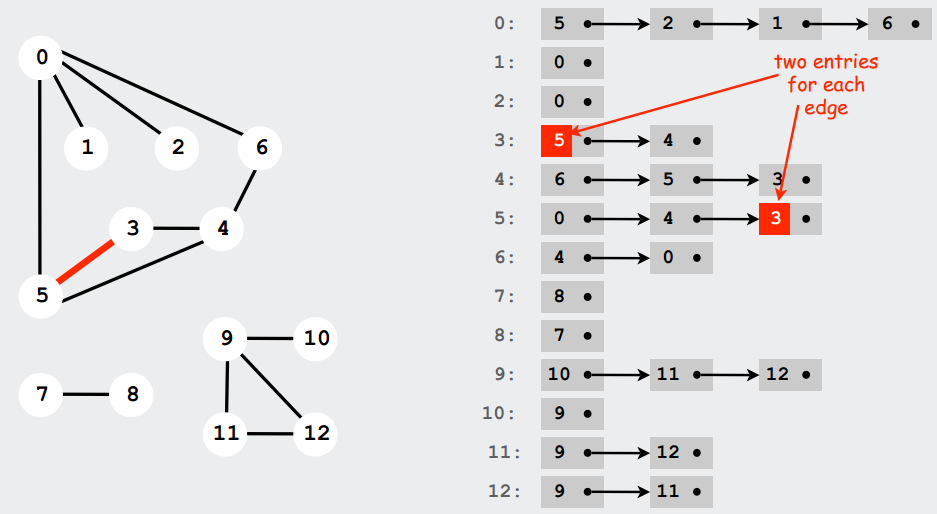
\includegraphics[width=0.9\textwidth]{figs/graph_dfs.png}
\end{frame}

\begin{frame}[fragile]
  \frametitle{DFS算法分析}
  \begin{itemize}
  \item 比较两种存储结构下的算法 (设 n 个顶点, e 条边)
    \begin{itemize}
    \item 数组表示:查找每个顶点的邻接点要遍历每一行,遍历的时间复杂度为$O(n^2)$
    \item 邻接表表示:虽然有 $2e$个表结点,但只需扫描$e$个结点即可完成遍历,加上访
      问$n$个头结点的时间,遍历的时间复杂度为$O(n+e)$
    \end{itemize}
  \item 结论:
    \begin{itemize}
    \item 稠密图适于在邻接矩阵上进行深度遍历;
    \item 稀疏图适于在邻接表上进行深度遍历。
    \end{itemize}
  \end{itemize}
\end{frame}

\begin{frame}[fragile]
  \frametitle{广度优先搜索 - Breadth First Search}
\begin{columns}[T]
    \column{0.65\textwidth}
    \scalebox{0.8}{
      \begin{tikzpicture}[scale=1]
        \GraphInit[vstyle=Normal]
        \SetVertexMath
        \Vertex{v_1}
        \Vertex[x=-2, y=-1]{v_2}
        \Vertex[x=1.5, y=-1]{v_3}

        \SOWE(v_2){v_4}
        \SOEA(v_2){v_5}


        \SOWE(v_3){v_6}
        \SOEA(v_3){v_7}
        \SOWE(v_5){v_8}

        \Edges(v_1,v_2,v_4,v_8,v_5,v_2)
        \Edges(v_1,v_3,v_6,v_7,v_3)
      \end{tikzpicture}
    }

    \scalebox{0.8}{
      \begin{tikzpicture}[ n/.style={minimum size=0.8cm}]
        \draw node[] (n0) {};
        \foreach \x  [evaluate = \x as \xp using int(\x-1)] in {1, ..., 8}
        \draw node[n, right=0 of n\xp](n\x) {$v_\x$};

        \foreach \x/\y in {1/1,2/0,3/0,4/0,5/0, 6/0, 7/0, 8/0}
        \draw node[n, below=0 of n\x, draw, fill=red!5](d\x) {$\y$};

        \draw node[left=0 of d1]{$visited$};

        \foreach \x/\y in {1/v_2,2/v_3,3/,4/,5/, 6/, 7/, 8/}
        \draw node[n, below=0.3 of d\x, draw, fill=yellow!20](d\x) {$\y$};

        \draw node[left=0 of d1]{$queue$};
      \end{tikzpicture}
    }
    
    \column{0.35\textwidth}
    \begin{tabular}{| l | l |}
      \hline
      $v_1$ & $\rightarrow v_2 \rightarrow v_3$ \\ \hline
      $v_2$ & $\rightarrow v_1 \rightarrow v_4 \rightarrow v_5$ \\ \hline
      $v_3$ & $\rightarrow v_1 \rightarrow v_6 \rightarrow v_7$ \\ \hline
      $v_4$ & $\rightarrow v_2 \rightarrow v_8$ \\ \hline
      $v_5$ & $\rightarrow v_2 \rightarrow v_8$ \\ \hline
      $v_6$ & $\rightarrow v_3 \rightarrow v_7$ \\ \hline
      $v_7$ & $\rightarrow v_3 \rightarrow v_6$ \\ \hline
      $v_8$ & $\rightarrow v_4 \rightarrow v_5$ \\ \hline      
    \end{tabular}
  \end{columns}

  \pause
  
  $v_1 \rightarrow v_2 \rightarrow v_3 \rightarrow v_4
  \rightarrow v_5 \rightarrow v_6 \rightarrow v_7 \rightarrow v_8$  
\end{frame}

\begin{frame}[allowframebreaks, fragile]
  \frametitle{BFS}

  \begin{minted}[fontsize=\small]{java}
    void bfs() {
      boolean[] visited = new boolean[vertices.length];
      //for (int i = 0; i < visited.length; i++) visited[i] = false;

      Queue<Integer> Q = new LinkedList<>();
      for (int v = 0; v < vertices.length; v++) {
        if (!visited[v]) {
          visited[v] = true;
          System.out.print(vertices[v].data + " ");
          Q.add(v);

          while (!Q.isEmpty()) {
            int u = Q.poll();

            for (EdgeNode w = vertices[u].firstAdj; w != null; w = w.nextAdj) {
              if (!visited[w.adjVertexNode]) {
                visited[w.adjVertexNode] = true;
                System.out.print(vertices[w.adjVertexNode].data + " ");
                Q.add(w.adjVertexNode);
              }
            }
          }
        }
      }
    }
  \end{minted}  
\end{frame}

\begin{frame}[fragile, allowframebreaks]
  \frametitle{分析以下代码的输出结果}
  
 \begin{minted}[fontsize=\small]{java}
    void bfs() {
        boolean[] visited = new boolean[vertices.length];
        //for (int i = 0; i < visited.length; i++) visited[i] = false;

        Queue<Integer> Q = new LinkedList<>();
        for (int v = 0; v < vertices.length; v++) {
            if (!visited[v]) {
                Q.add(v);
            }

            while (!Q.isEmpty()) {
                int u = Q.poll();

                visited[u] = true;
                System.out.print(vertices[u].data + " ");

                for (EdgeNode w = vertices[u].firstAdj; w != null; w = w.nextAdj) {
                    if (!visited[w.adjVertexNode]) {
                        Q.add(w.adjVertexNode);
                    }
                }
            }
        }
    }
 \end{minted}
\end{frame}

\begin{frame}[fragile]
  \frametitle{BFS算法分析}
  \begin{itemize}
  \item 数组表示:BFS对于每一个被访问到的顶点,都要循环检测矩阵中的整整一行(n个元
    素),总的时间代价为$O(n^2)$
  \item 邻接表表示:时间复杂度$O(n+e)$
  \end{itemize}
\end{frame}

\begin{frame}[fragile]
  \frametitle{作业练习}
  \begin{enumerate}
  \item 请写出如下有向图的邻接矩阵,基于该矩阵进行图的深度优先遍历;
  \item 建立如下有向图的邻接表,进行图的广度优先遍历.
  \end{enumerate}

  \scalebox{0.8}{
    \begin{tikzpicture}[scale=1.5]
      \GraphInit[vstyle=Normal]
      \SetVertexMath

      \Vertex{3} \NOWE(3){0} \NOEA(3){1} \SOWE(3){5} \SOEA(3){6} 

      \Vertex[x=-2, y=0] {2} 	\Vertex[x=2, y=0] {4}

      \Edges[style={-Latex}](0,1,4,6,5)
      \Edges[style={-Latex}](0,2,5)
      \Edges[style={-Latex}](0,3,5)
      \Edges[style={-Latex}](1,3,6)
      \Edges[style={-Latex}](4,3,2)
    \end{tikzpicture}
  }
\end{frame}


\subsection{图的连通性}
\begin{frame}[fragile]
  \frametitle{图的连通性}

  图的连通性在计算机网、通信网和电力网等方面有着重要的应用。
\end{frame}

\begin{frame}[fragile]
  \frametitle{生成树(Spanning tree)}
  \begin{columns}[T]
    \column{0.5\textwidth}
    深度优先生成树:

    \scalebox{0.8}{      
      \begin{tikzpicture}[scale=1]
        \GraphInit[vstyle=Normal]
        \SetVertexMath
        \Vertex{v_1}
        \Vertex[x=-2, y=-1]{v_2}
        \Vertex[x=1.5, y=-1]{v_3}

        \SOWE(v_2){v_4}
        \SOEA(v_2){v_5}


        \SOWE(v_3){v_6}
        \SOEA(v_3){v_7}
        \SOWE(v_5){v_8}

        \Edges[color=red](v_1,v_2,v_4,v_8,v_5,v_2)
        \Edges[color=red](v_1,v_3,v_6,v_7,v_3)
        \Edges(v_3,v_7)
        \Edges(v_2,v_5)
      \end{tikzpicture}   
    }
    \column{0.5\textwidth}
    广度优先生成树:

    \scalebox{0.8}{      
      \begin{tikzpicture}[scale=1]
        \GraphInit[vstyle=Normal]
        \SetVertexMath
        \Vertex{v_1}
        \Vertex[x=-2, y=-1]{v_2}
        \Vertex[x=1.5, y=-1]{v_3}

        \SOWE(v_2){v_4}
        \SOEA(v_2){v_5}


        \SOWE(v_3){v_6}
        \SOEA(v_3){v_7}
        \SOWE(v_5){v_8}

        \Edges[color=red](v_1,v_2,v_4,v_8,v_5,v_2)
        \Edges[color=red](v_1,v_3,v_6,v_7,v_3)
        \Edges(v_5,v_8)
        \Edges(v_6,v_7)
      \end{tikzpicture}   
    }
  \end{columns}
  连通图的生成树是它的极小连通子图,有$n$个顶点和$n-1$条边。
\end{frame}

\begin{frame}[fragile]
  \frametitle{非连通图的连通分量}

  对于非连通图则遍历生成森林, 下图是深度优先遍历生成森林

  \scalebox{0.8}{    
    \begin{tikzpicture}[scale=1]
      \GraphInit[vstyle=Normal]
      \SetVertexMath
      \Vertex{v_1}
      \Vertex[x=-2, y=-1]{v_2}
      \Vertex[x=1.5, y=-1]{v_3}

      \SOWE(v_2){v_4}
      \SOEA(v_2){v_5}


      \SOWE(v_3){v_6}
      \SOEA(v_3){v_7}
      \SOWE(v_5){v_8}

      \Edges[color=red](v_2,v_4,v_8,v_5,v_2)
      \Edges[color=red](v_1,v_3,v_6,v_7,v_3)
      \Edges(v_3,v_7)
      \Edges(v_2,v_5)
    \end{tikzpicture}   
  }
\end{frame}

\begin{frame}[fragile]
  \frametitle{最小生成树}
  \begin{itemize}
  \item 很多现实问题可以抽象成网。比如,在$n$个城市之间建立通信网,要求总成本最低。
  \item 上述问题是求连通网的最小生成树问题,即挑选$n-1$条不产生回路的最短边,则总成
    本(生成树的各边的权重之和)达到最低。
  \end{itemize}

  \begin{columns}[T]
    \column{0.5\textwidth}
    \scalebox{0.8} {
      \begin{tikzpicture}[n/.style={draw, circle, minimum size=0.5cm}]
        \draw node[n](v3){$v_3$} node[n, above=of v3] (v1) {$v_1$}
        node[n, left=of v3, xshift=-0.5cm,yshift=0.5cm] (v2) {$v_2$} node[n, right=of v3, xshift=0.5cm, yshift=0.5cm] (v4) {$v_4$}
        node[n, below left=of v3] (v5) {$v_5$} node[n, below right=of v3] (v6) {$v_6$};
        \path[draw] (v1) edge node[above]{6} (v2) 
        (v1) edge node[right]{1} (v3) 
        (v1) edge node[above]{5} (v4) 
        (v2) edge node[above]{5} (v3) 
        (v2) edge node[left]{3} (v5) 
        (v4) edge node[above]{5} (v3) 
        (v4) edge node[left]{2} (v6) 
        (v5) edge node[above]{6} (v3) 
        (v5) edge node[above]{6} (v6) 
        (v6) edge node[right] {4} (v3);

        \draw[draw=red!50,thick] (v1) -- (v3) --(v5) --(v2) (v3) --(v6) --(v4);

        \draw node[below=2 of v3]{总成本为16};
      \end{tikzpicture}
    }

    \column{0.5\textwidth}
    \scalebox{0.8}{
      \begin{tikzpicture}[n/.style={draw, circle, minimum size=0.5cm}]
        \draw node[n](v3){$v_3$} node[n, above=of v3] (v1) {$v_1$}
        node[n, left=of v3, xshift=-0.5cm,yshift=0.5cm] (v2) {$v_2$} node[n, right=of v3, xshift=0.5cm, yshift=0.5cm] (v4) {$v_4$}
        node[n, below left=of v3] (v5) {$v_5$} node[n, below right=of v3] (v6) {$v_6$};

        \path[draw] (v1) edge node[above]{6} (v2) 
        (v1) edge node[right]{1} (v3) 
        (v1) edge node[above]{5} (v4) 
        (v2) edge node[above]{5} (v3) 
        (v2) edge node[left]{3} (v5) 
        (v4) edge node[above]{5} (v3) 
        (v4) edge node[left]{2} (v6) 
        (v5) edge node[above]{6} (v3) 
        (v5) edge node[above]{6} (v6) 
        (v6) edge node[right] {4} (v3);

        \draw[draw=red!50,thick] (v3) -- (v1) --(v2) --(v5) -- (v6) --(v4) --(v1);

        \draw node[below=2 of v3]{总成本为23};
      \end{tikzpicture}      
    }
  \end{columns}
\end{frame}

\begin{frame}[fragile, allowframebreaks]
  \frametitle{Prim MST}
  \begin{minted}[fontsize=\scriptsize]{java}
    public class PrimMST {
      static int minimum(CloseEdge[] closeEdges) {
        int minValue = closeEdges[0].lowcost;
        int minVex = 0;
        for (int i = 1; i < closeEdges.length; i++) {
          int lowcost = closeEdges[i].lowcost;
          if (lowcost > 0 && (lowcost < minValue || minValue == 0)) {
            minValue = lowcost;
            minVex = i;
          }
        }
        return minVex;
      }

      static void mst() {
        CloseEdge[] closeEdges = new CloseEdge[Graph.vexnum];
        closeEdges[0] = new CloseEdge(0, 0);

        //初始化
        for (int i = 1; i < Graph.vexnum; i++) {
          closeEdges[i] = new CloseEdge(0, Graph.arcs[0][i]);
        }

        //默认选中了第0个节点,处理剩余的n-1个
        for (int i = 1; i < Graph.vexnum; i++) {
          int k = minimum(closeEdges);
          String fromVex = Graph.labels[closeEdges[k].adjvex];
          String toVex = Graph.labels[k];

          System.out.println(fromVex + " -> " + toVex);
          closeEdges[k].lowcost = 0;

          //处理每一个Vertex, 看能否通过k让代价更低
          for (int j = 0; j < Graph.vexnum; j++) {
            if (Graph.arcs[k][j] < closeEdges[j].lowcost) {
              closeEdges[j].lowcost = Graph.arcs[k][j];
              closeEdges[j].adjvex = k;
            }
          }
        }
      }

      public static void main(String[] args) {
        mst();
      }

      public static class CloseEdge {
        public int adjvex;
        public int lowcost;

        public CloseEdge(int adjvex, int lowcost) {
          this.adjvex = adjvex;
          this.lowcost = lowcost;
        }
      }


      public static class Graph {
        public static int INFINITE = 10000;

        public static int vexnum = 6;

        public static String[] labels = new String[]{"v1", "v2", "v3",
          "v4", "v5", "v6"};

        public static int[][] arcs = new int[][]{
          {0, 6, 1, 5, INFINITE, INFINITE},
          {6, 0, 5, INFINITE, 3, INFINITE},
          {1, 5, 0, 5, 6, 4},
          {5, INFINITE, 5, 0, INFINITE, 2},
          {0, 3, 6, INFINITE, 0, 6},
          {INFINITE, INFINITE, 4, 2, 6, 0}
        };
      }
    }
  \end{minted}
\end{frame}


\begin{frame}[fragile]
  \frametitle{本章作业}
  \begin{enumerate}
  \item 最小生成树的Prim, Kruscal算法
  \item 最短路径的Dijstra, Floyd算法
  \end{enumerate}

  \begin{itemize}
  \item 编程实现上述算法(务必认真写注释),
  \item 要求显示某图的最小生成树/某两点之间的最短路径;
  \item 基本要求:Prim, Kruscal可以二选一, Dijstra, Floyd可以二选一
  \item 优秀要求:四种算法都实现
  \end{itemize}
\end{frame}